\section{Setup}
\label{sec:setup}

Two different setups are used, in order to systematically provide an
independant cross check of the results:
\begin{itemize}
\item standalone simulation of a detector with a transverse size of $20 \times 20$cm$^2$ and 30 layers.
\item full geometry of the final detector in CMSSW.
\end{itemize}

For the standalone simulation, two different analyses are also run in
parallel and cross-checking each others systematically.

\subsection{The standalone simulation setup}
\label{sec:standalone}

This setup is used for three different purposes: provide a quick
handle to optimise the design parameters (see
section~\ref{sec:optim}), extract performance results in ideal
conditions, and cross-check the performances in pileup conditions with
the CMSSW setup. The code is available in git under the following
repository: \url{https://github.com/pfs/PFCal/}.

\subsubsection{Geant4 setup}

The detector construction is made of 30 sampling sections, each with
the following parameters:
\begin{table}{h!}
\caption{\label{tab:samplSec} Thicknesses (in mm) for the different materials, per layer}
\begin{tabular}{|l|c|c|c|c|c|}
\hline
Layers & Pb & Cu & Si & PCB & Air \\
\hline
1-10  & 1.63 & 3 & 0.2 & 1 & 2 \\
11-20 & 3.32 & 3 & 0.2 & 1 & 2 \\
21-30 & 5.56 & 3 & 0.2 & 1 & 2 \\
\hline
\end{tabular}
\end{table}

Figure~\ref{fig:g4vis} shows an event display of a 50 GeV electron
shower in two different geometries: a uniform 26 layers of 1 X$_0$
each (left) and the baseline geometry detailed in
table~\ref{tab:samplSec}.

\begin{figure}[h!]
  \begin{center}
    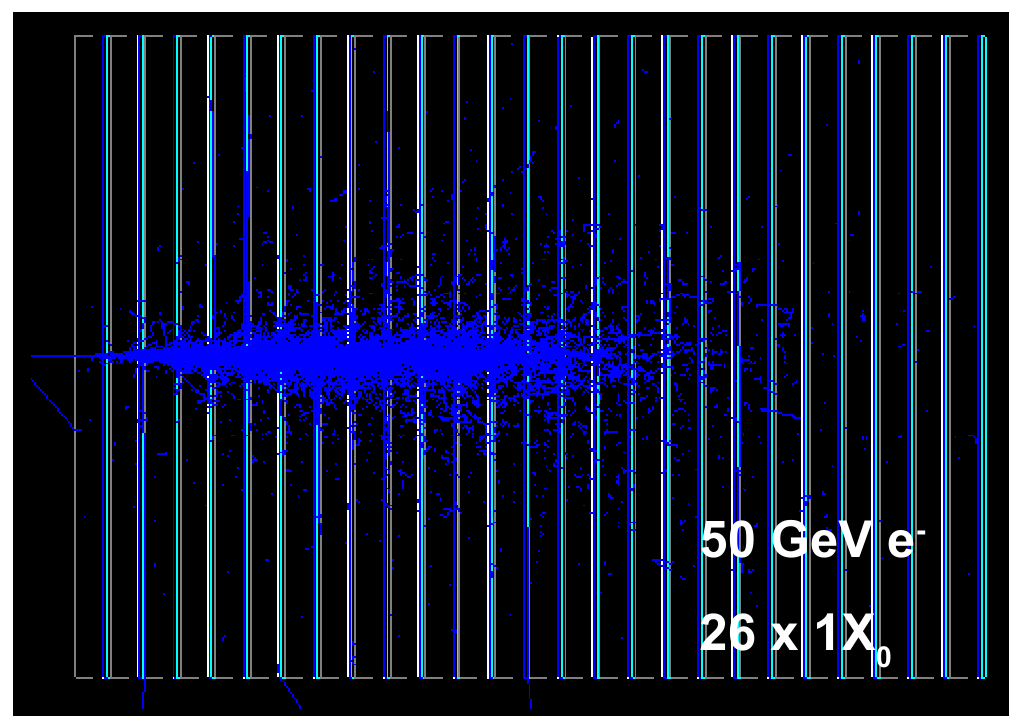
\includegraphics[width=\cmsFigWidth]{figures/e_50GeV_uniform_26x0.png}
    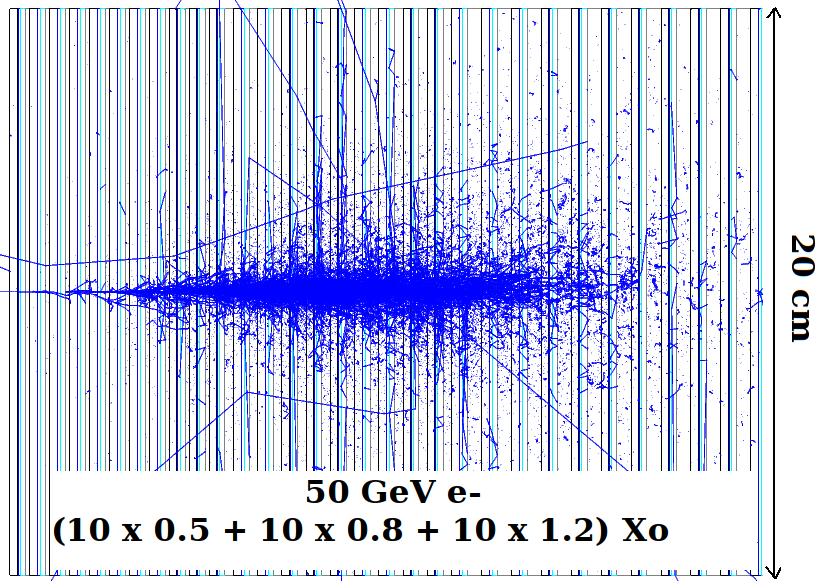
\includegraphics[width=\cmsFigWidth]{figures/e_50GeV_concept_v3.png}
    \caption{Event displays of a 50 GeV electron showers in the
      standalone simulation. Left: uniform 26 layers of 1 X$_0$
      each. Right: 30 layers in three blocks of different
      thicknesses. Electron deposits are shown in blue. Photons have
      been hidden for better visibility.}
    \label{fig:g4vis}
  \end{center}
\end{figure}

The simulation uses the QGSP\_BERT physics list, with the default cuts
for electrons, positrons and photons reduced to 10\,$\mu$m in the
silicon. The default elsewhere is 700\,$\mu$m. With 700\,$\mu$m in Si,
a 420 keV (5.8 keV) electron (photon) would deposit all its energy in
one step. With the reduced 10\,$\mu$m, the energy threshold is 32 keV
for electrons, and 990 eV for photons.



\subsubsection{Energy resolution}